\chapter{项目需求}

\section{系统背景}
在过去的几十年中,餐饮行业一直是人们生活中重要的组成部分。然而,随着城市化和工作压力的增加,传统的进餐方式面临着许多挑战。人们的时间日益宝贵,越来越多的人选择在家或办公室点外卖,以节省时间和精力。这为外卖平台的崛起提供了机会。随着智能手机的普及,移动互联网的兴起以及在线支付的便捷性,外卖平台逐渐演变成一个综合性的餐饮服务平台,为用户提供了更加便利、多样化的选择。

“饿了么”外卖平台为用户和餐厅提供了一个互相连接的桥梁,具有以下核心功能:
\begin{itemize}
    \item{\textbf{用户点餐}}:用户通过“饿了么”移动应用程序或网站浏览附近的餐厅和菜单,并可以根据自己的口味和需求下订单。
    \item{\textbf{多样选择}}:平台上的餐厅涵盖了各种菜系,从传统美食到国际化的料理,满足了用户不同的口味偏好。
    \item{\textbf{配送服务}}:“饿了么”为用户提供送餐服务,用户可以实时跟踪订单状态,知道餐食的准确送达时间。
    \item{\textbf{在线支付}}:用户可以通过平台进行在线支付,不需要现金交易,实现O2O(Online~to~Offline)外卖模式
    \item{\textbf{评价和评论}}:用户可以对餐厅和菜品进行评价和评论,帮助其他用户做出更好的选择。
    \item{\textbf{营销活动}}:平台定期推出各种促销活动和优惠券,吸引用户下单并提升用户粘性。
\end{itemize}

\section{系统架构}
\subsection{饿了么外卖平台系统架构描述}
本软件采用前后端分离的开发方式,为移动端开发一个外卖平台软件。
\begin{itemize}
    \item {数据库}:
    \item {后端}:
    \item {前端}:首先采用~HTML5、~CSS3~和~JavaScript~语言的相关技术开发外卖平台的静态页面。其次采用~Vue3~架构构造一个与后端交互的前端页面。
\end{itemize}
\subsection{饿了么外卖平台系统架构图}

\section{业务架构}
\subsection{用户点餐业务流程描述}
首先,用户在首页选择了相应的商家分类,便会跳转至对应的商家列表页面。在商家页表页面里,用户选择相应的商家并跳转至对应的商家信息页面。在商家信息页面里,用户可以选择往购物车里添加或删除菜品。当用户选择完毕,并会跳转至确认订单页面。

在确认订单页面中,用户可以选择送货地址以及检查自己的订单是否正确,确认无误后就会跳转至在线支付页面。在此页面中,用户可以选择不同的第三方支付方式并确认支付。点餐业务到此结束。
\subsection{用户点餐业务流程图}
本软件的用户点餐流程图如图~\ref{fig:process}~所示。
\begin{figure}[htbp]
    \centering
    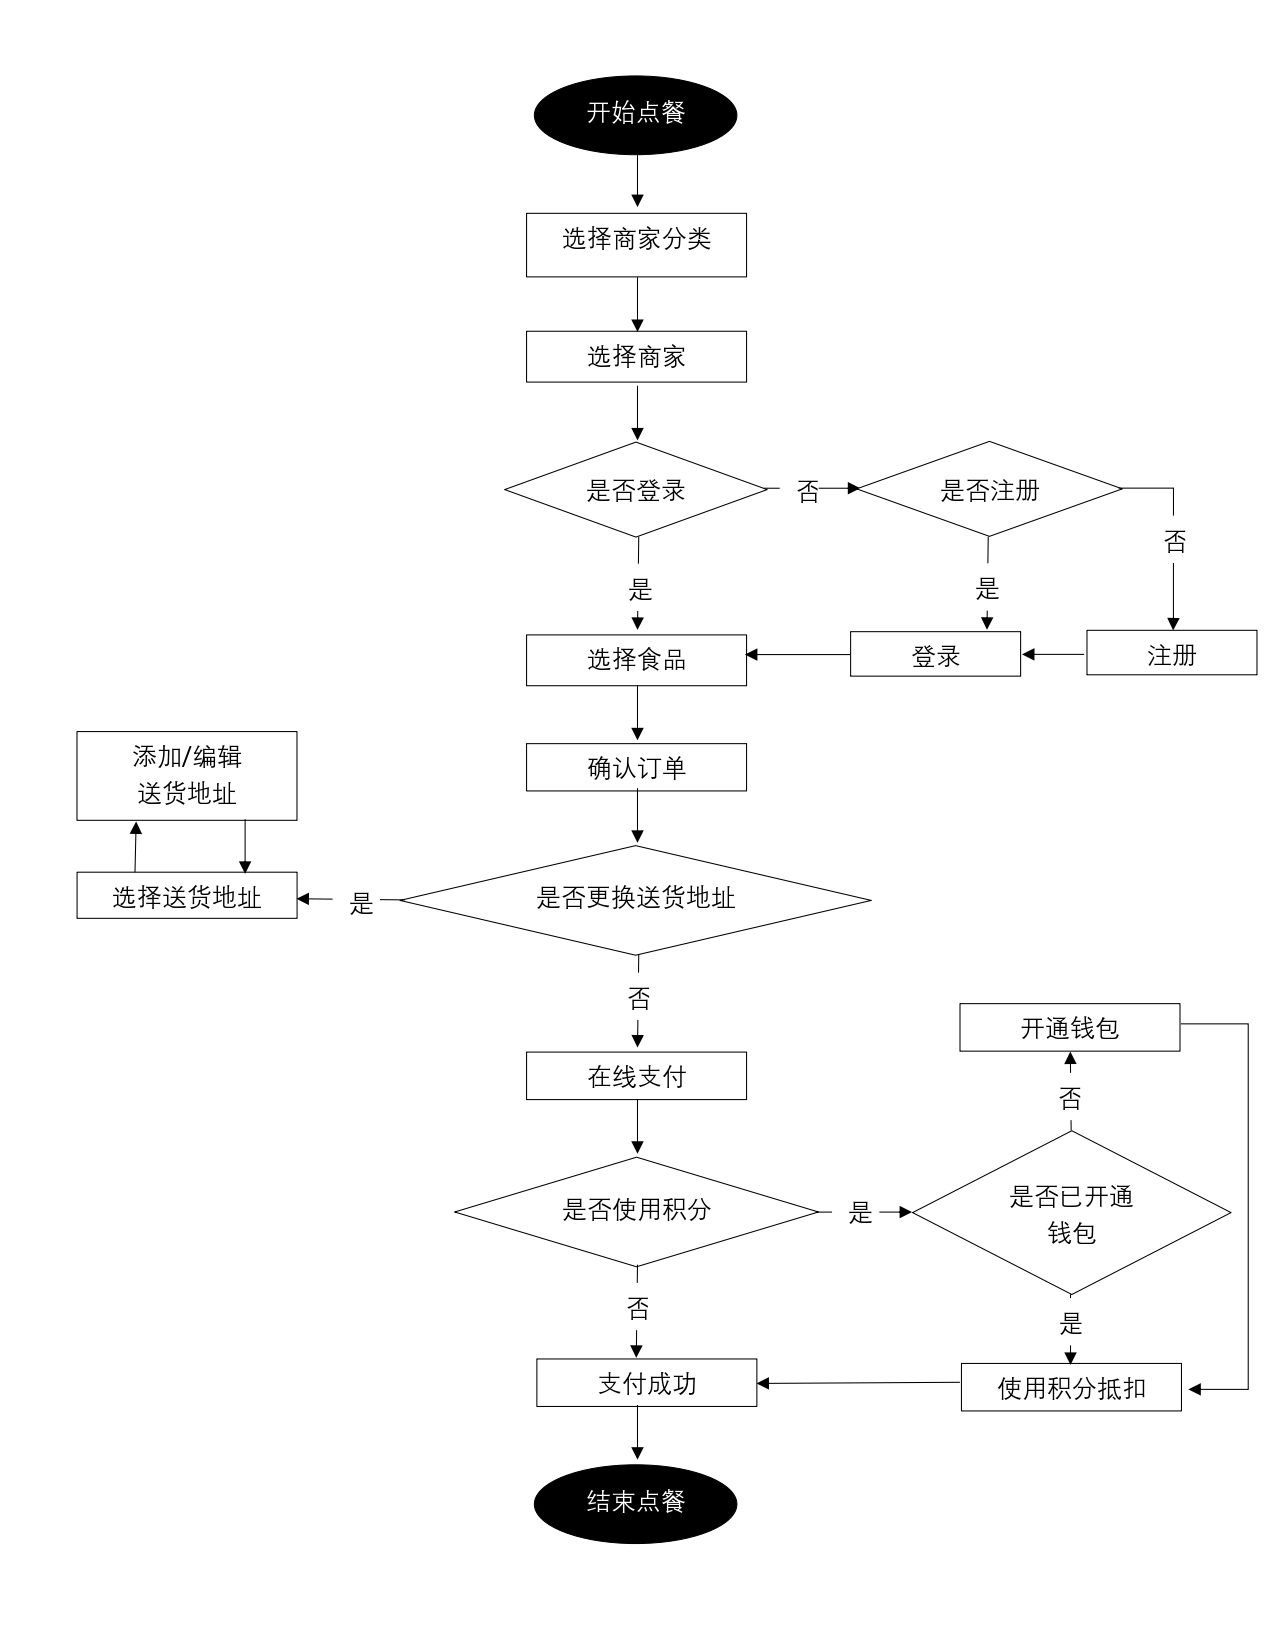
\includegraphics[width=0.8\textwidth]{processmap}
    \caption{饿了么外卖平台用户点餐业务流程图}\label{fig:process}
    \vspace{\baselineskip}
    \end{figure}

\section{用户需求}
本软件由三个用户组成,分别为用户、商家和管理员。用户角色由表~\ref{tab:table1}~所示。
\begin{table}[htbp]
\caption{饿了么外卖平台不同用户的功能描述}\label{tab:table1}
\vspace{0.5em}\wuhao
\begin{tabularx}{\textwidth}{llX}
\toprule[1.5pt]
序号 & 用户 & 功能描述 \\ 
\midrule[1pt]
1 & 用户 & 
\begin{itemize}
    \item{\textbf{游览菜品}}:消费者可以在首页浏览附近的餐厅列表。他们可以按照菜系、评分、特别优惠等条件筛选餐厅,了解每家餐厅的菜单和菜品详情。
    \item{\textbf{选择菜品}}:消费者可以根据菜品的图片、描述以及价格做出最合适的选择。
    \item{\textbf{在线支付}}:消费者将所选的菜品添加到购物车,确认订单后选择第三方的支付方式进行支付,完成订单。
    \item {\textbf{管理地址信息}}:消费者可以自行添加、删除和查看收获地址的信息。
    \item {\textbf{管理订单信息}}:消费者可以在历史订单页面查看已生成的订单状态,其中包含已选购的商家和菜品明细。
    \item {\textbf{登陆注册}}:消费者可以通过手机号注册一个饿了么外卖平台的账号。
\end{itemize}
\\
2 & 商家 & 
\begin{itemize}
    \item{\textbf{注册和上架}}:商家需要先在平台上注册自己的餐厅。一旦注册成功,他们可以填写餐厅的基本信息、菜单、菜品描述和价格等。
    \item{\textbf{菜单管理}}:商家可以通过平台管理菜单,包括添加新菜品、修改菜品信息、调整价格等。
    \item{\textbf{接受订单}}:商家在平台上收到订单通知后,可以查看订单详情,包括所点菜品、数量、送达地址以及支付信息。
    \item {\textbf{准备食物}}:商家接受订单后,就可以开始准备食物。
\end{itemize}
\\
3 & 管理员 & 
\begin{itemize}
    \item{\textbf{平台监督和管理}}:管理员负责监督外卖平台的整体运营情况。他们使用管理后台工具,监控平台的性能、稳定性和安全性,确保用户能够顺利访问平台。
    \item{\textbf{监控订单和投诉}}:管理员跟踪订单处理流程,确保订单按时送达。
    \item{\textbf{技术支持和升级}}:管理员负责监督技术团队,确保平台的技术架构和功能持续适应市场需求,并在必要时进行系统更新。
    \item {\textbf{风险管理和安全性}}:管理员制定隐私政策、安全措施,确保用户的个人信息和支付数据得到妥善保护。
\end{itemize}
\\
\bottomrule[1.5pt]
\end{tabularx}
\vspace{\baselineskip}
\end{table}

\section{功能性需求}
\subsection{首页}
首页是本软件的主要页面。此页面展示了用户当前的收货地址、商家搜索栏、菜品分类、推荐商家列表以及其他优惠部分。首页的底部有一个菜单,显示外卖平台的【首页】、【发现】、【订单】以及【我的】按钮。用户可以点击相应的按钮跳转至对应的页面进行操作。
\subsubsection{界面设计}
本软件的首页界面设计如图~\ref{fig:index}~所示。
\begin{figure}[htbp]
\centering
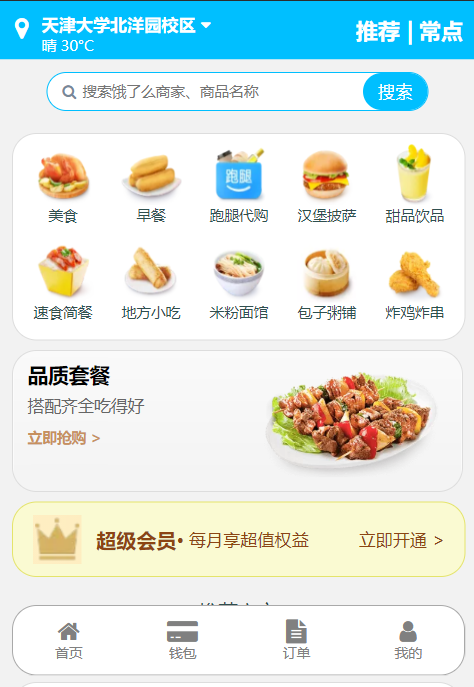
\includegraphics[width=0.4\textwidth]{index}
\caption{首页界面设计}\label{fig:index}
\vspace{\baselineskip}
\end{figure}
\subsubsection{功能按钮}
本软件首页功能按钮如表~\ref{tab:table2}~所示。
\begin{table}[htbp]
    \caption{饿了么外卖平台首页功能按钮}\label{tab:table2}
    \vspace{0.5em}\wuhao
    \begin{tabularx}{\textwidth}{lllX}
    \toprule[1.5pt]
    序号 & 按钮名称 & 功能 & 功能规则 \\ 
    \midrule[1pt]
    1 & 当前送货地址 & 用户选择送货地址 & 点击跳转至地址管理页面。 \\
    2 & 搜索框 & 用户搜索商家名称 & 输入商家名称可根据商家名称查找商家。 \\
    3 & 商家分类 & 用户选择商家分类 & 点击跳转指定商家分类。 \\
    4 & 首页 & 刷新页面 & 点击跳转至首页。 \\
    5 & 订单 & 进入历史订单 & 点击跳转至历史订单页面。 \\
    6 & 我的 & 进入用户信息 & 点击跳转至用户信息页面。 \\
\bottomrule[1.5pt]
\end{tabularx}
\vspace{\baselineskip}
\end{table}

\subsection{商家列表}
当用户在首页点击指定的商家分类后,会跳转至指定分类的商家列表页面。此页面展示了一系列商家,其中包括他们的商家图片、商家名称、商家的起送费、配送费和菜品。
\subsubsection{界面设计}
本软件的商家列表界面设计如图~\ref{fig:businessList}~所示。
\begin{figure}[htbp]
\centering
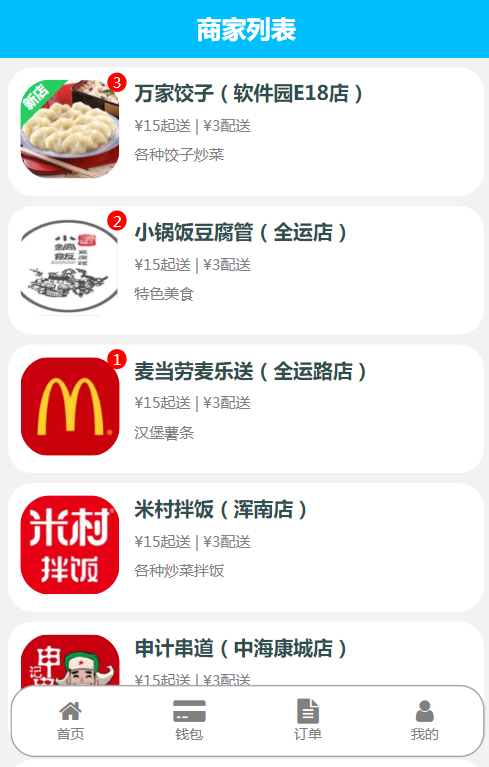
\includegraphics[width=0.4\textwidth]{businessList}
\caption{商家列表界面设计}\label{fig:businessList}
\vspace{\baselineskip}
\end{figure}
\subsubsection{功能按钮}
本软件商家列表功能按钮如表~\ref{tab:table3}~所示。
\begin{table}[htbp]
    \caption{饿了么外卖平台商家列表功能按钮}\label{tab:table3}
    \vspace{0.5em}\wuhao
    \begin{tabularx}{\textwidth}{lllX}
    \toprule[1.5pt]
    序号 & 按钮名称 & 功能 & 功能规则 \\ 
    \midrule[1pt]
    1 & 商家信息 & 用户选择指定商家 & 点击跳转至指定商家信息页面。 \\
    2 & 首页 & 刷新页面 & 点击跳转至首页。 \\
    3 & 订单 & 进入历史订单 & 点击跳转至历史订单页面。 \\
    4 & 我的 & 进入用户信息 & 点击跳转至用户信息页面。 \\
\bottomrule[1.5pt]
\end{tabularx}
\vspace{\baselineskip}
\end{table}

\subsection{商家信息}
当用户在商家列表页面中点击指定的商家后,会跳转至该商家的信息页面。此页面展示了该商家的图片、名称、起送费、配送费以及该商家一系列的菜品。此页面的下方显示了当前购物车的菜品数量、总价格以及【去结算】的按钮。
\subsubsection{界面设计}
本软件的商家信息界面设计如图~\ref{fig:businessInfo}~所示。
\begin{figure}[htbp]
\centering
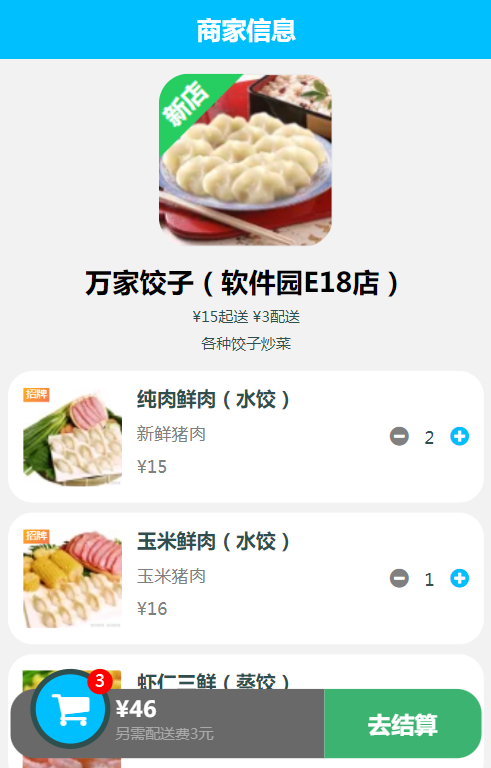
\includegraphics[width=0.4\textwidth]{businessInfo}
\caption{商家信息界面设计}\label{fig:businessInfo}
\vspace{\baselineskip}
\end{figure}
\subsubsection{功能按钮}
本软件商家信息功能按钮如表~\ref{tab:table4}~所示。
\begin{table}[htbp]
    \caption{饿了么外卖平台商家信息功能按钮}\label{tab:table4}
    \vspace{0.5em}\wuhao
    \begin{tabularx}{\textwidth}{lllX}
    \toprule[1.5pt]
    序号 & 按钮名称 & 功能 & 功能规则 \\ 
    \midrule[1pt]
    1 & 添加菜品 & 用户添加该菜品数量 & 点击将该菜品在购物车里的数量加1。 \\
    2 & 减少菜品 & 用户减少该菜品数量 & 点击将该菜品在购物车里的数量减1。 \\
    3 & 去结算 & 进入确认订单页面 & 点击会生成订单,跳转至确认订单页面。 \\
\bottomrule[1.5pt]
\end{tabularx}
\vspace{\baselineskip}
\end{table}

\subsection{确认订单}
当用户在商家信息页面中点击【去结算】按钮后,会跳转至确认订单页面。此页面展示了当前用户的送货地址、用户名称和手机号。在用户信息的下方显示了商家名称、购物车中所选择的菜品图片、菜品名称、菜品数量和配送费。在此页面的底部显示了总价格和【去支付】的按钮。
\subsubsection{界面设计}
本软件的确认订单界面设计如图~\ref{fig:order}~所示。
\begin{figure}[htbp]
\centering
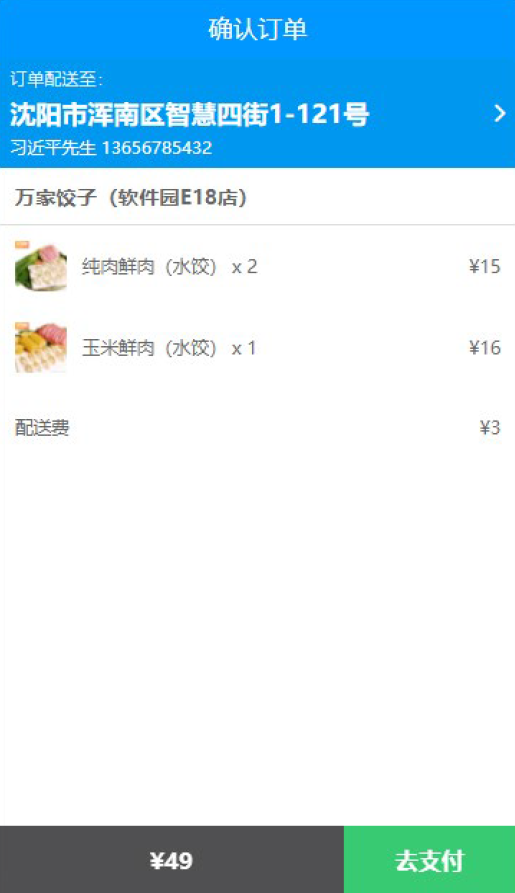
\includegraphics[width=0.4\textwidth]{order}
\caption{确认订单界面设计}\label{fig:order}
\vspace{\baselineskip}
\end{figure}
\subsubsection{功能按钮}
本软件确认订单功能按钮如表~\ref{tab:table5}~所示。
\begin{table}[htbp]
    \caption{饿了么外卖平台确认订单功能按钮}\label{tab:table5}
    \vspace{0.5em}\wuhao
    \begin{tabularx}{\textwidth}{lllX}
    \toprule[1.5pt]
    序号 & 按钮名称 & 功能 & 功能规则 \\ 
    \midrule[1pt]
    1 & 当前送货地址 & 用户选择送货地址 & 点击跳转至地址管理页面。 \\
    2 & 去支付 & 进入在线支付页面 & 点击跳转至在线支付页面。 \\
\bottomrule[1.5pt]
\end{tabularx}
\vspace{\baselineskip}
\end{table}

\subsection{在线支付}
当用户在确认订单页面中点击【去结算】按钮后,会跳转至确认订单页面。
\subsubsection{界面设计}
本软件的在线支付界面设计如图~\ref{fig:payment}~所示。
\begin{figure}[htbp]
\centering
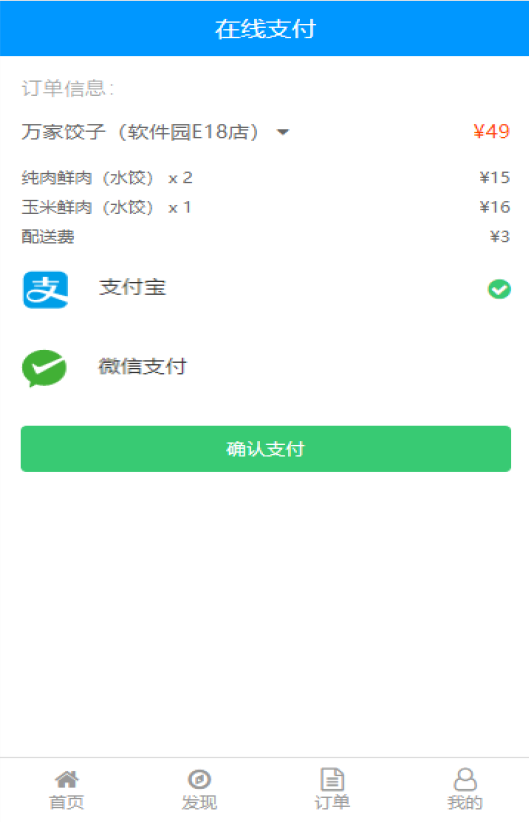
\includegraphics[width=0.4\textwidth]{payment}
\caption{在线支付界面设计}\label{fig:payment}
\vspace{\baselineskip}
\end{figure}
\subsubsection{功能按钮}
本软件在线支付功能按钮如表~\ref{tab:table6}~所示。
\begin{table}[htbp]
    \caption{饿了么外卖平台在线支付功能按钮}\label{tab:table6}
    \vspace{0.5em}\wuhao
    \begin{tabularx}{\textwidth}{lllX}
    \toprule[1.5pt]
    序号 & 按钮名称 & 功能 & 功能规则 \\ 
    \midrule[1pt]
    1 & 箭头 & 用户展开订单明细 & 点击展开已生成的订单明细,包括菜品的数量和价格。 \\
    2 & 选择支付方式 & 用户选择第三方的支付方式 & 点击选择任一第三方支付方式。 \\
    3 & 确认支付 & 用户支付订单 & 点击完成点餐流程。 \\
    4 & 首页 & 进入首页 & 点击跳转至首页。 \\
    5 & 订单 & 进入历史订单 & 点击跳转至历史订单页面。 \\
    6 & 我的 & 进入用户信息 & 点击跳转至用户信息页面。 \\
\bottomrule[1.5pt]
\end{tabularx}
\vspace{\baselineskip}
\end{table}

\subsection{用户登录}
此页面为用户登录的页面。用户需要输入手机号和密码,若两者正确无误则登陆成功并跳转至上一个页面,否则服务器将会提示信息错误。
\subsubsection{界面设计}
本软件的用户登录界面设计如图~\ref{fig:login}~所示。
\begin{figure}[htbp]
\centering
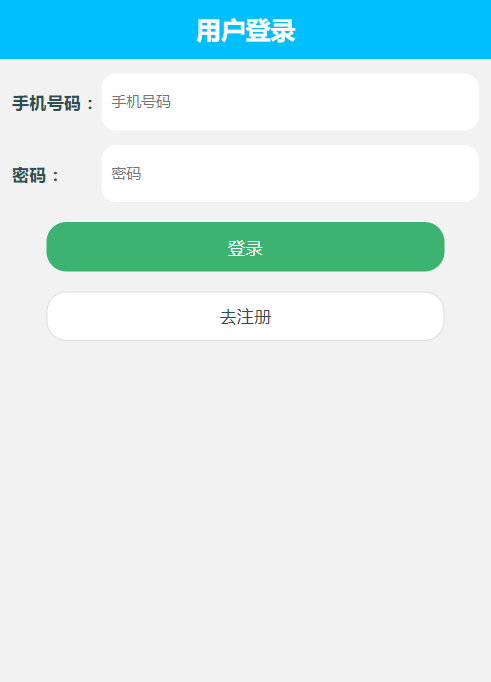
\includegraphics[width=0.4\textwidth]{login}
\caption{用户登录界面设计}\label{fig:login}
\vspace{\baselineskip}
\end{figure}
\subsubsection{功能按钮}
本软件用户登录功能按钮如表~\ref{tab:table7}~所示。
\begin{table}[htbp]
    \caption{饿了么外卖平台用户登录功能按钮}\label{tab:table7}
    \vspace{0.5em}\wuhao
    \begin{tabularx}{\textwidth}{lllX}
    \toprule[1.5pt]
    序号 & 按钮名称 & 功能 & 功能规则 \\ 
    \midrule[1pt]
    1 & 登录 & 用户登录 & 若手登陆成功则跳转至上一个页面,否则服务器将会显示错误提示。 \\
    2 & 去注册 & 用户注册 & 点击跳转至用户注册页面。 \\
    3 & 首页 & 进入首页 & 点击跳转至首页。 \\
    4 & 订单 & 进入历史订单 & 点击跳转至历史订单页面。 \\
    5 & 我的 & 进入用户信息 & 点击跳转至用户信息页面。 \\
\bottomrule[1.5pt]
\end{tabularx}
\vspace{\baselineskip}
\end{table}

\subsection{用户注册}
此页面为用户注册的页面。用户需要输入手机号、两次相同的密码、用户姓名以及选择性别。若手机号、密码和用户名都符合要求,则注册成功并跳转至登陆页面,否则服务器将会提示信息错误。
\subsubsection{界面设计}
本软件的用户注册界面设计如图~\ref{fig:register}~所示。
\begin{figure}[htbp]
\centering
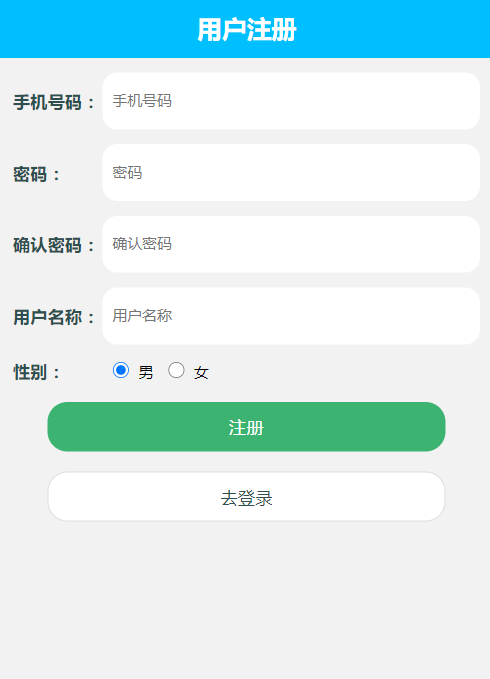
\includegraphics[width=0.4\textwidth]{register}
\caption{用户注册界面设计}\label{fig:register}
\vspace{\baselineskip}
\end{figure}
\subsubsection{功能按钮}
本软件用户注册功能按钮如表~\ref{tab:table8}~所示。
\begin{table}[htbp]
    \caption{饿了么外卖平台用户注册功能按钮}\label{tab:table8}
    \vspace{0.5em}\wuhao
    \begin{tabularx}{\textwidth}{lllX}
    \toprule[1.5pt]
    序号 & 按钮名称 & 功能 & 功能规则 \\ 
    \midrule[1pt]
    1 & 性别 & 用户选择性别 & 点击选择任一性别。 \\
    2 & 注册 & 用户注册 & 若注册成功则跳转至登陆页面,否则服务器将显示错误提示。 \\
    3 & 首页 & 进入首页 & 点击跳转至首页。 \\
    4 & 订单 & 进入历史订单 & 点击跳转至历史订单页面。 \\
    5 & 我的 & 进入用户信息 & 点击跳转至用户信息页面。 \\
\bottomrule[1.5pt]
\end{tabularx}
\vspace{\baselineskip}
\end{table}

\subsection{历史订单}
历史订单页面展示了用户之前所生成的全部订单,未支付的订单会显示在页面的上方,已支付的订单则会显示在页面的下方。
\subsubsection{界面设计}
本软件的历史订单界面设计如图~\ref{fig:orderList}~所示。
\begin{figure}[htbp]
\centering
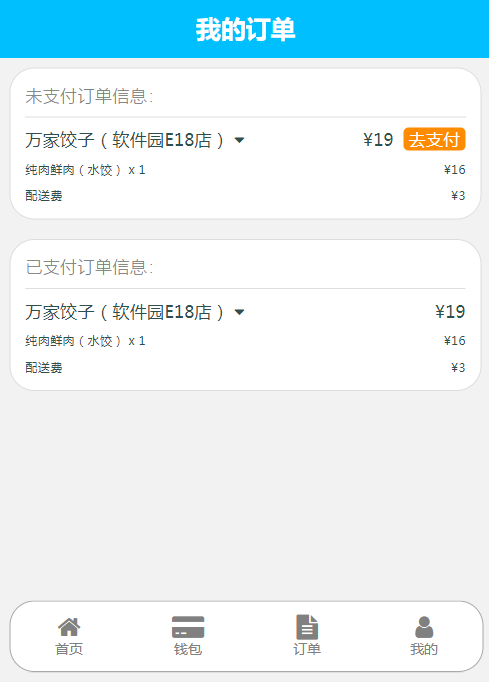
\includegraphics[width=0.4\textwidth]{orderList}
\caption{历史订单界面设计}\label{fig:orderList}
\vspace{\baselineskip}
\end{figure}
\subsubsection{功能按钮}
本软件历史订单功能按钮如表~\ref{tab:table9}~所示。
\begin{table}[htbp]
    \caption{饿了么外卖平台历史订单功能按钮}\label{tab:table9}
    \vspace{0.5em}\wuhao
    \begin{tabularx}{\textwidth}{lllX}
    \toprule[1.5pt]
    序号 & 按钮名称 & 功能 & 功能规则 \\ 
    \midrule[1pt]
    1 & 箭头 & 用户展开订单明细 & 点击展开已生成的订单明细,包括菜品的数量和价格。 \\
    2 & 去支付 & 用户支付未支付的订单 & 点击跳转至未支付的订单页面。 \\
    3 & 首页 & 进入首页 & 点击跳转至首页。 \\
    4 & 订单 & 刷新页面 & 点击跳转至历史订单页面。 \\
    5 & 我的 & 进入用户信息 & 点击跳转至用户信息页面。 \\
\bottomrule[1.5pt]
\end{tabularx}
\vspace{\baselineskip}
\end{table}

\subsection{地址管理}
当用户在首页或在确认订单页面点击送货地址按钮时,会跳转到此页面。此页面显示了用户的所有送货地址。
\subsubsection{界面设计}
本软件的地址管理界面设计如图~\ref{fig:userAddress}~所示。
\begin{figure}[htbp]
\centering
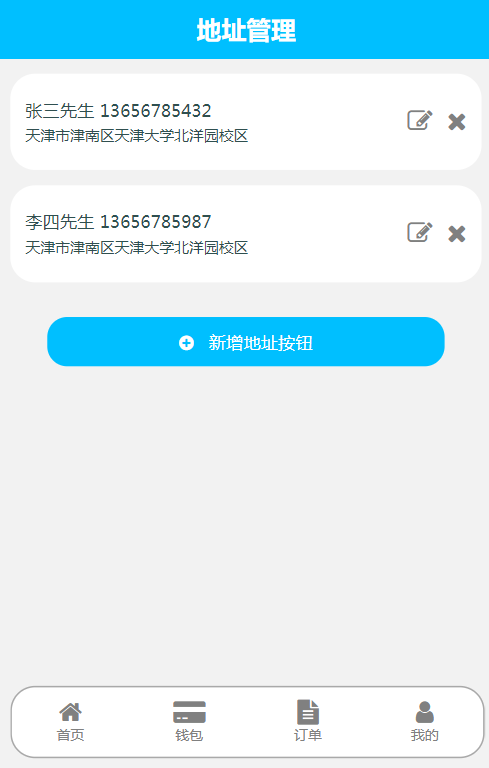
\includegraphics[width=0.4\textwidth]{userAddress}
\caption{地址管理界面设计}\label{fig:userAddress}
\vspace{\baselineskip}
\end{figure}
\subsubsection{功能按钮}
本软件地址管理功能按钮如表~\ref{tab:table10}~所示。
\begin{table}[htbp]
    \caption{饿了么外卖平台地址管理功能按钮}\label{tab:table10}
    \vspace{0.5em}\wuhao
    \begin{tabularx}{\textwidth}{lllX}
    \toprule[1.5pt]
    序号 & 按钮名称 & 功能 & 功能规则 \\ 
    \midrule[1pt]
    1 & 送货地址 & 用户选择该送货地址 & 点击选择该送货地址,并跳转至上一个页面。 \\
    2 & 编辑图标 & 用户编辑该送货地址 & 点击跳转至编辑送货地址页面。 \\
    3 & 打叉图标 & 用户删除该送货地址 & 点击删除该送货地址,地址管理页面减少该送货地址。 \\
    4 & 新增收货地址 & 用户添加送货地址 & 点击跳转至新增送货地址页面。 \\
    5 & 首页 & 进入首页 & 点击跳转至首页。 \\
    6 & 订单 & 进入历史订单 & 点击跳转至历史订单页面。 \\
    7 & 我的 & 进入用户信息 & 点击跳转至用户信息页面。 \\
\bottomrule[1.5pt]
\end{tabularx}
\vspace{\baselineskip}
\end{table}

\subsection{新增送货地址}
用户在此页面添加新的送货地址。填写完成后,点击保存按钮跳转至地址管理页面。
\subsubsection{界面设计}
本软件的新增送货地址界面设计如图~\ref{fig:addUserAddress}~所示。
\begin{figure}[htbp]
\centering
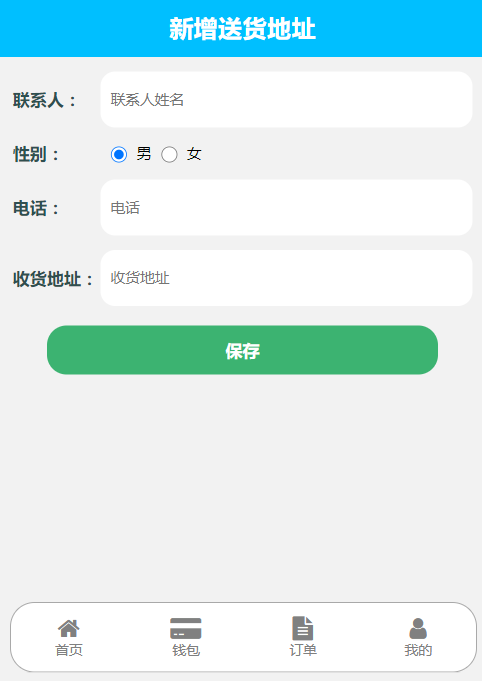
\includegraphics[width=0.4\textwidth]{addUserAddress}
\caption{新增送货地址界面设计}\label{fig:addUserAddress}
\vspace{\baselineskip}
\end{figure}
\subsubsection{功能按钮}
本软件新增送货地址功能按钮如表~\ref{tab:table11}~所示。
\begin{table}[htbp]
    \caption{饿了么外卖平台新增送货地址功能按钮}\label{tab:table11}
    \vspace{0.5em}\wuhao
    \begin{tabularx}{\textwidth}{lllX}
    \toprule[1.5pt]
    序号 & 按钮名称 & 功能 & 功能规则 \\ 
    \midrule[1pt]
    1 & 性别 & 用户选择性别 & 点击选择任一性别。 \\
    2 & 保存 & 用户保存当前送货地址 & 点击跳转至地址管理页面。 \\
    3 & 首页 & 进入首页 & 点击跳转至首页。 \\
    4 & 订单 & 进入历史订单 & 点击跳转至历史订单页面。 \\
    5 & 我的 & 进入用户信息 & 点击跳转至用户信息页面。 \\
\bottomrule[1.5pt]
\end{tabularx}
\vspace{\baselineskip}
\end{table}

\subsection{编辑地址}
用户在此页面编辑已选择的送货地址。填写完成后,点击保存按钮跳转至地址管理页面。
\subsubsection{界面设计}
本软件的编辑送货地址界面设计如图~\ref{fig:editUserAddress}~所示。
\begin{figure}[htbp]
\centering
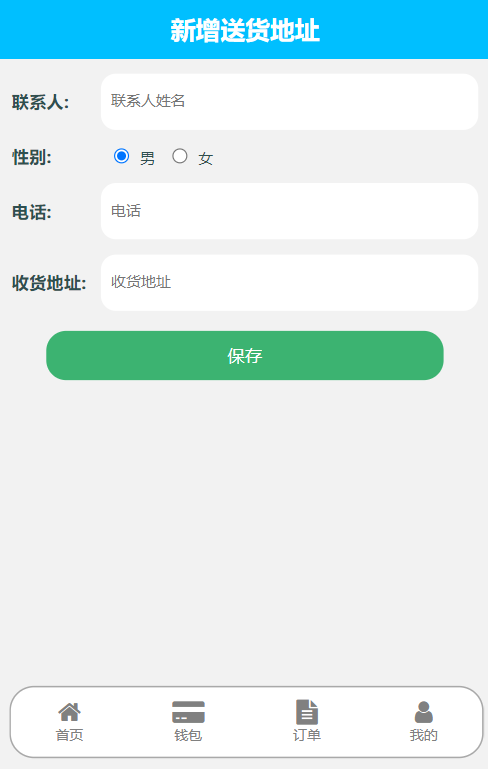
\includegraphics[width=0.4\textwidth]{editUserAddress}
\caption{编辑送货地址界面设计}\label{fig:editUserAddress}
\vspace{\baselineskip}
\end{figure}
\subsubsection{功能按钮}
本软件编辑送货地址功能按钮如表~\ref{tab:table12}~所示。
\begin{table}[htbp]
    \caption{饿了么外卖平台编辑送货地址功能按钮}\label{tab:table12}
    \vspace{0.5em}\wuhao
    \begin{tabularx}{\textwidth}{lllX}
    \toprule[1.5pt]
    序号 & 按钮名称 & 功能 & 功能规则 \\ 
    \midrule[1pt]
    1 & 性别 & 用户选择性别 & 点击选择任一性别。 \\
    2 & 保存 & 用户保存当前送货地址 & 点击跳转至地址管理页面。 \\
    3 & 首页 & 进入首页 & 点击跳转至首页。 \\
    4 & 订单 & 进入历史订单 & 点击跳转至历史订单页面。 \\
    5 & 我的 & 进入用户信息 & 点击跳转至用户信息页面。 \\
\bottomrule[1.5pt]
\end{tabularx}
\vspace{\baselineskip}
\end{table}

\subsection{个人信息}
个人信息页面显示当前用户的图片和名称。用户可以在此页面修改用户名和密码、跳转至地址管理页面以及退出登录。
\subsubsection{界面设计}
本软件的个人信息界面设计如图~\ref{fig:profile}~所示。
\begin{figure}[htbp]
\centering
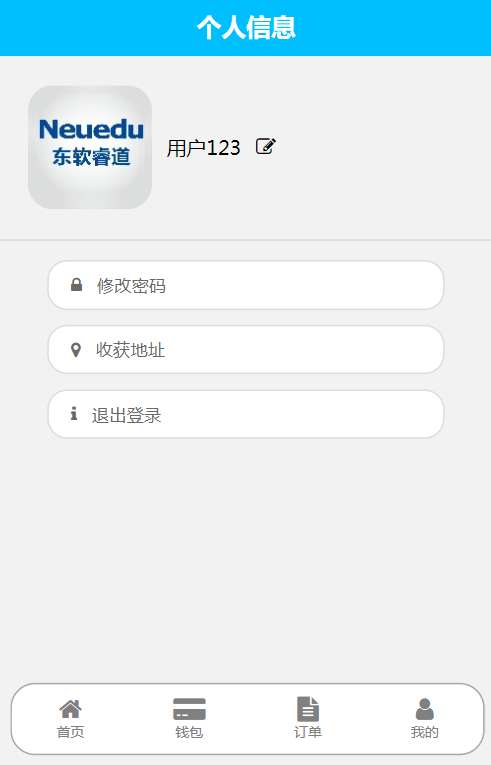
\includegraphics[width=0.4\textwidth]{profile}
\caption{个人信息界面设计}\label{fig:profile}
\vspace{\baselineskip}
\end{figure}
\subsubsection{功能按钮}
本软件编辑送货地址功能按钮如表~\ref{tab:table13}~所示。
\begin{table}[htbp]
    \caption{饿了么外卖平台编辑送货地址功能按钮}\label{tab:table13}
    \vspace{0.5em}\wuhao
    \begin{tabularx}{\textwidth}{lllX}
    \toprule[1.5pt]
    序号 & 按钮名称 & 功能 & 功能规则 \\ 
    \midrule[1pt]
    1 & 编辑图标 & 进入更新用户名页面 & 点击跳转至更新用户名页面。 \\
    2 & 修改密码 & 进入更新密码页面 & 点击跳转至更新密码页面。 \\
    3 & 收货地址 & 进入地址管理页面 & 点击跳转至地址管理页面。 \\
    4 & 退出登录 & 进入首页 & 点击退出登录,跳转至首页。 \\
    5 & 首页 & 进入首页 & 点击跳转至首页。 \\
    6 & 订单 & 进入历史订单页面 & 点击跳转至历史订单页面。 \\
    7 & 我的 & 刷新页面 & 点击跳转至用户信息页面。 \\
\bottomrule[1.5pt]
\end{tabularx}
\vspace{\baselineskip}
\end{table}

\subsection{更新用户名}
用户在此页面更新用户名。填写完成后,点击保存按钮跳转至个人信息页面。
\subsubsection{界面设计}
本软件的更新用户名界面设计如图~\ref{fig:updateUserName}~所示。
\begin{figure}[htbp]
\centering
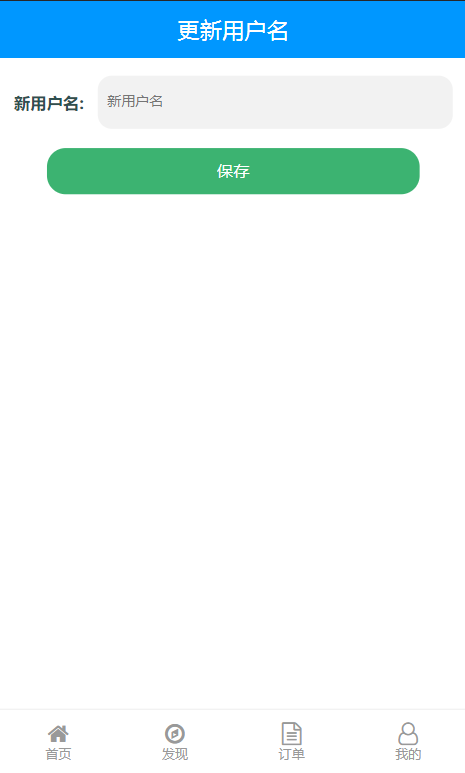
\includegraphics[width=0.4\textwidth]{updateUserName}
\caption{更新用户名界面设计}\label{fig:updateUserName}
\vspace{\baselineskip}
\end{figure}
\subsubsection{功能按钮}
本软件更新用户名功能按钮如表~\ref{tab:table14}~所示。
\begin{table}[htbp]
    \caption{饿了么外卖平台更新用户名功能按钮}\label{tab:table14}
    \vspace{0.5em}\wuhao
    \begin{tabularx}{\textwidth}{lllX}
    \toprule[1.5pt]
    序号 & 按钮名称 & 功能 & 功能规则 \\ 
    \midrule[1pt]
    1 & 保存 & 用户保存当前用户名 & 点击跳转至个人信息页面。 \\
    2 & 首页 & 进入首页 & 点击跳转至首页。 \\
    3 & 订单 & 进入历史订单页面 & 点击跳转至历史订单页面。 \\
    4 & 我的 & 刷新页面 & 点击跳转至用户信息页面。 \\
\bottomrule[1.5pt]
\end{tabularx}
\vspace{\baselineskip}
\end{table}

\subsection{更新密码}
用户在此页面更新密码。填写完成后,点击保存按钮跳转至个人信息页面。
\subsubsection{界面设计}
本软件的更新密码界面设计如图~\ref{fig:updateUserPassword}~所示。
\begin{figure}[htbp]
\centering
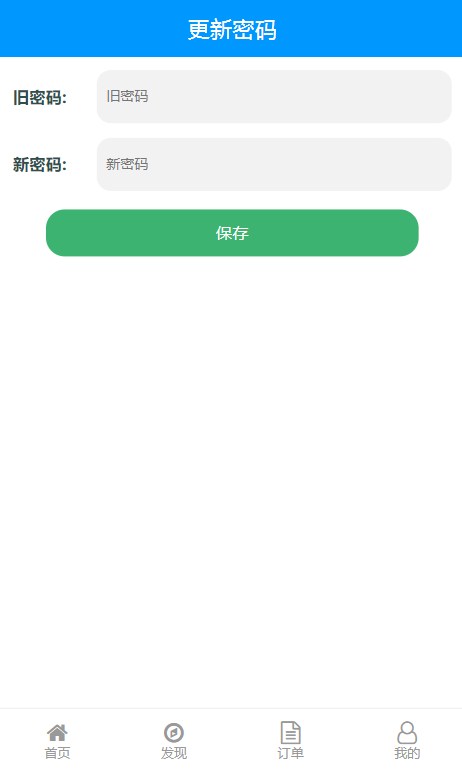
\includegraphics[width=0.4\textwidth]{updateUserPassword}
\caption{更新密码界面设计}\label{fig:updateUserPassword}
\vspace{\baselineskip}
\end{figure}
\subsubsection{功能按钮}
本软件更新密码功能按钮如表~\ref{tab:table15}~所示。
\begin{table}[htbp]
    \caption{饿了么外卖平台更新密码功能按钮}\label{tab:table15}
    \vspace{0.5em}\wuhao
    \begin{tabularx}{\textwidth}{lllX}
    \toprule[1.5pt]
    序号 & 按钮名称 & 功能 & 功能规则 \\ 
    \midrule[1pt]
    1 & 保存 & 用户保存当前密码 & 点击跳转至个人信息页面。 \\
    2 & 首页 & 进入首页 & 点击跳转至首页。 \\
    3 & 订单 & 进入历史订单页面 & 点击跳转至历史订单页面。 \\
    4 & 我的 & 刷新页面 & 点击跳转至用户信息页面。 \\
\bottomrule[1.5pt]
\end{tabularx}
\vspace{\baselineskip}
\end{table}